\documentclass[oneside, a4paper, 12pt]{book}
\usepackage[ngerman]{babel}
\usepackage{graphicx}
\usepackage{calc}
\usepackage{fancyvrb}
\pagestyle{empty}
\usepackage[utf8]{inputenc}
\usepackage{array}
\inputencoding{utf8}
%\usepackage[absolute,showboxes]{textpos}
\usepackage[absolute]{textpos}
\usepackage{amssymb}

\usepackage[]{eso-pic}[2002/11/16]

\usepackage{fancybox} % fuer Oval...

%\usepackage{showframe}


\setlength{\tabcolsep}{0.2cm}
\setlength{\topmargin}{1cm}
\setlength{\parindent}{0pt}

\newlength{\Rand}
\setlength{\Rand}{\oddsidemargin + \hoffset + 1in}

\begin{document}
\fontfamily{phv}\selectfont
\textblockorigin{0cm}{0cm}

\newlength{\Logo}
\setlength{\Logo}{210mm-60mm}
\begin{textblock*}{\Logo}(30mm,10mm)%

\includegraphics[width=\Logo]{pcars-main.png}
\end{textblock*}

\begin{textblock*}{\Logo}(30mm,125mm)%
\begin{center}\Huge{Project CARS Tracks}\end{center}
\end{textblock*}

\begin{textblock*}{90mm}(120mm,275mm)%
\begin{center}\Huge{22. May 2015}\end{center}
\end{textblock*}

\begin{textblock*}{90mm}(0mm,275mm)%
\begin{center}\tt{https://github.com/wwwutz/pCars-Tracks}\end{center}
\end{textblock*}

\begin{textblock*}{30mm}(0mm,0mm)%

\includegraphics[width=30mm]{LG/2015-05-20_00094.png}
\end{textblock*}
\begin{textblock*}{30mm}(30mm,0mm)%

\includegraphics[width=30mm]{LG/2015-05-20_00086.png}
\end{textblock*}
\begin{textblock*}{30mm}(60mm,0mm)%

\includegraphics[width=30mm]{LG/2015-05-20_00072.png}
\end{textblock*}
\begin{textblock*}{30mm}(90mm,0mm)%

\includegraphics[width=30mm]{LG/2015-05-20_00076.png}
\end{textblock*}
\begin{textblock*}{30mm}(120mm,0mm)%

\includegraphics[width=30mm]{LG/2015-05-20_00089.png}
\end{textblock*}
\begin{textblock*}{30mm}(150mm,0mm)%

\includegraphics[width=30mm]{LG/2015-05-20_00074.png}
\end{textblock*}
\begin{textblock*}{30mm}(180mm,0mm)%

\includegraphics[width=30mm]{LG/2015-05-20_00092.png}
\end{textblock*}
\begin{textblock*}{30mm}(0mm,30mm)%

\includegraphics[width=30mm]{LG/2015-05-20_00080.png}
\end{textblock*}
\begin{textblock*}{30mm}(180mm,30mm)%

\includegraphics[width=30mm]{LG/2015-05-20_00091.png}
\end{textblock*}
\begin{textblock*}{30mm}(0mm,60mm)%

\includegraphics[width=30mm]{LG/2015-05-20_00097.png}
\end{textblock*}
\begin{textblock*}{30mm}(180mm,60mm)%

\includegraphics[width=30mm]{LG/2015-05-20_00081.png}
\end{textblock*}
\begin{textblock*}{30mm}(0mm,90mm)%

\includegraphics[width=30mm]{LG/2015-05-20_00087.png}
\end{textblock*}
\begin{textblock*}{30mm}(180mm,90mm)%

\includegraphics[width=30mm]{LG/2015-05-20_00083.png}
\end{textblock*}
\begin{textblock*}{30mm}(0mm,120mm)%

\includegraphics[width=30mm]{LG/2015-05-20_00085.png}
\end{textblock*}
\begin{textblock*}{30mm}(180mm,120mm)%

\includegraphics[width=30mm]{LG/2015-05-20_00079.png}
\end{textblock*}
\begin{textblock*}{30mm}(30mm,150mm)%

\includegraphics[width=30mm]{LG/2015-05-20_00100.png}
\end{textblock*}
\begin{textblock*}{30mm}(90mm,150mm)%

\includegraphics[width=30mm]{LG/2015-05-20_00096.png}
\end{textblock*}
\begin{textblock*}{30mm}(150mm,150mm)%

\includegraphics[width=30mm]{LG/2015-05-20_00099.png}
\end{textblock*}
\begin{textblock*}{30mm}(0mm,180mm)%
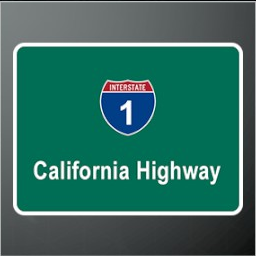
\includegraphics[width=30mm]{LG/2015-05-20_00077.png}
\end{textblock*}
\begin{textblock*}{30mm}(60mm,180mm)%

\includegraphics[width=30mm]{LG/2015-05-20_00098.png}
\end{textblock*}
\begin{textblock*}{30mm}(120mm,180mm)%

\includegraphics[width=30mm]{LG/2015-05-20_00075.png}
\end{textblock*}
\begin{textblock*}{30mm}(180mm,180mm)%
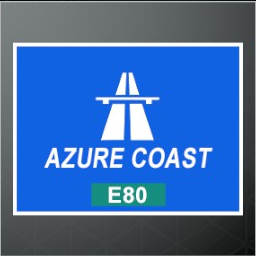
\includegraphics[width=30mm]{LG/2015-05-20_00073.png}
\end{textblock*}
\begin{textblock*}{30mm}(30mm,210mm)%

\includegraphics[width=30mm]{LG/2015-05-20_00082.png}
\end{textblock*}
\begin{textblock*}{30mm}(90mm,210mm)%

\includegraphics[width=30mm]{LG/2015-05-20_00078.png}
\end{textblock*}
\begin{textblock*}{30mm}(150mm,210mm)%

\includegraphics[width=30mm]{LG/2015-05-20_00095.png}
\end{textblock*}
\begin{textblock*}{30mm}(0mm,240mm)%

\includegraphics[width=30mm]{LG/2015-05-20_00088.png}
\end{textblock*}
\begin{textblock*}{30mm}(60mm,240mm)%

\includegraphics[width=30mm]{LG/2015-05-20_00093.png}
\end{textblock*}
\begin{textblock*}{30mm}(120mm,240mm)%

\includegraphics[width=30mm]{LG/2015-05-20_00090.png}
\end{textblock*}
\begin{textblock*}{30mm}(180mm,240mm)%

\includegraphics[width=30mm]{LG/2015-05-20_00084.png}
\end{textblock*}

\null\newpage

\begin{textblock*}{60mm}(15mm,15mm)%

\includegraphics[width=50mm]{LG/2015-05-20_00086.png}
\par Autodromo Nazionale Monza\\ Italy
\end{textblock*}
\begin{textblock*}{80mm}(85mm,15mm)%
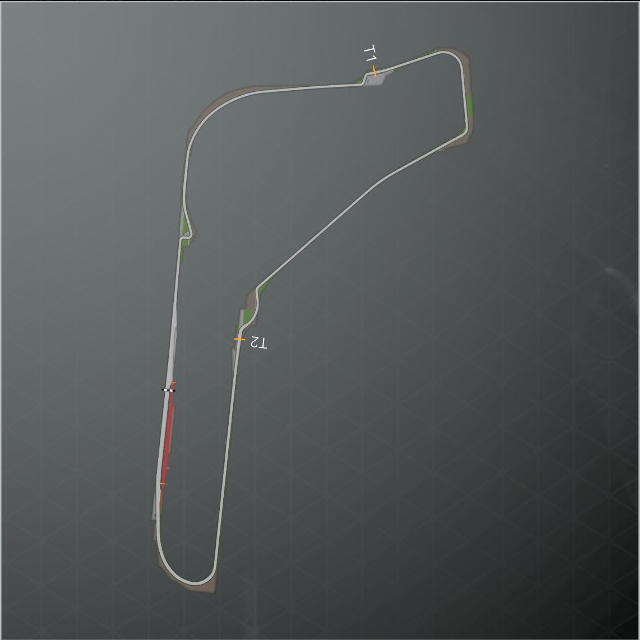
\includegraphics[width=80mm]{TR/2015-05-20_00034.png}
\centerline{Autodromo Nazionale Monza GP}
\par\hfill\tiny\tt ANMOGP\\
\end{textblock*}
\begin{textblock*}{30mm}(170mm,15mm)%
\par \Huge$\circlearrowleft$
\Large
\par$\mapsto$ 3.59 mi.
\par$\mapsto$ 5.78 km
\par$\looparrowright$ 11
\end{textblock*}
\begin{textblock*}{80mm}(85mm,105mm)%
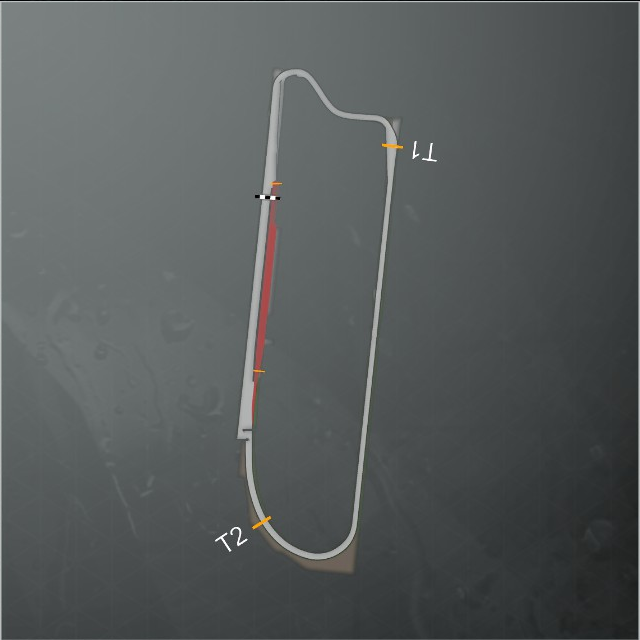
\includegraphics[width=80mm]{TR/2015-05-20_00035.png}
\centerline{Autodromo Nazionale Monza Short}
\par\hfill\tiny\tt ANMOSH\\
\end{textblock*}
\begin{textblock*}{30mm}(170mm,105mm)%
\par \Huge$\circlearrowleft$
\Large
\par$\mapsto$ 1.52 mi.
\par$\mapsto$ 2.45 km
\par$\looparrowright$ 6
\end{textblock*}
\begin{textblock*}{60mm}(15mm,195mm)%

\includegraphics[width=50mm]{LG/2015-05-20_00072.png}
\par Azure Circuit\\ France
\end{textblock*}
\begin{textblock*}{80mm}(85mm,195mm)%
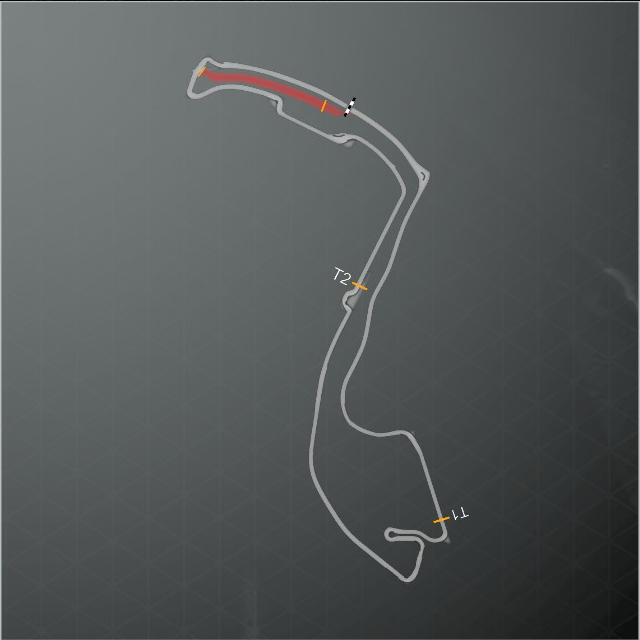
\includegraphics[width=80mm]{TR/2015-05-20_00001.png}
\centerline{Azure Circuit}
\par\hfill\tiny\tt AZCI\\
\end{textblock*}
\begin{textblock*}{30mm}(170mm,195mm)%
\par \Huge$\circlearrowleft$
\Large
\par$\mapsto$ 2.07 mi.
\par$\mapsto$ 3.33 km
\par$\looparrowright$ 19
\end{textblock*}
\null\newpage

\begin{textblock*}{60mm}(15mm,15mm)%
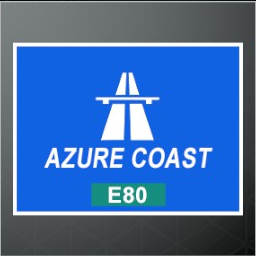
\includegraphics[width=50mm]{LG/2015-05-20_00073.png}
\par Azure Coast\\ France
\end{textblock*}
\begin{textblock*}{80mm}(85mm,15mm)%
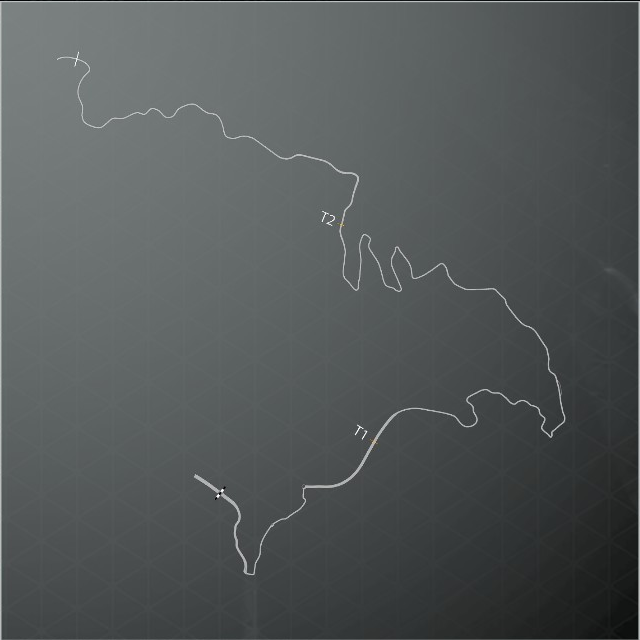
\includegraphics[width=80mm]{TR/2015-05-20_00002.png}
\centerline{Azure Coast}
\par\hfill\tiny\tt AZCO\\
\end{textblock*}
\begin{textblock*}{30mm}(170mm,15mm)%
\par A $\rightsquigarrow$ B
\Large
\par$\mapsto$ 11.96 mi.
\par$\mapsto$ 19.25 km
\par$\looparrowright$ 95
\end{textblock*}
\begin{textblock*}{80mm}(85mm,105mm)%
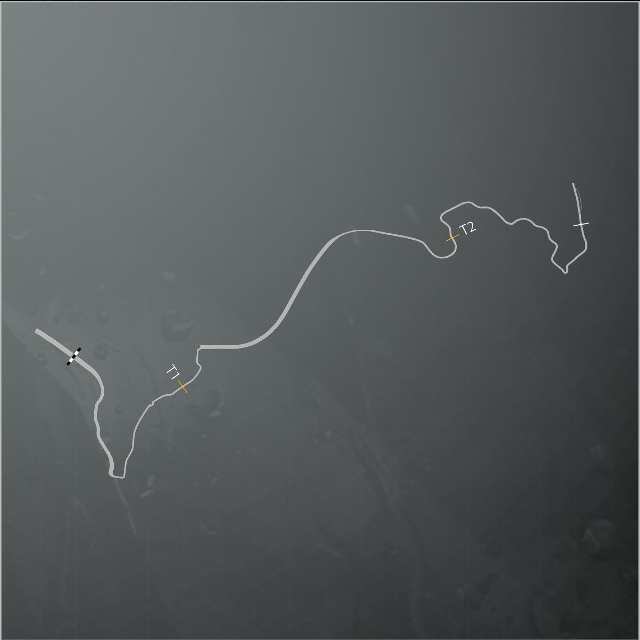
\includegraphics[width=80mm]{TR/2015-05-20_00003.png}
\centerline{Azure Coast Stage 1}
\par\hfill\tiny\tt AZCOS1\\
\end{textblock*}
\begin{textblock*}{30mm}(170mm,105mm)%
\par A $\rightsquigarrow$ B
\Large
\par$\mapsto$ 4.59 mi.
\par$\mapsto$ 7.39 km
\par$\looparrowright$ 40
\end{textblock*}
\begin{textblock*}{80mm}(85mm,195mm)%
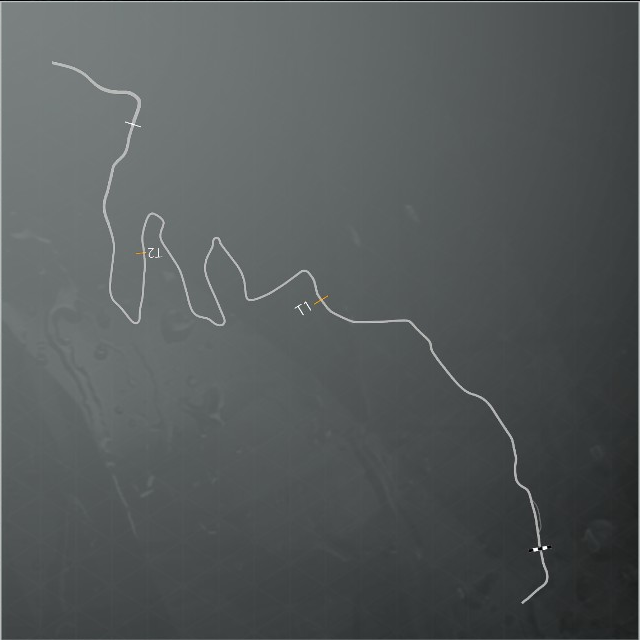
\includegraphics[width=80mm]{TR/2015-05-20_00004.png}
\centerline{Azure Coast Stage 2}
\par\hfill\tiny\tt AZCOS2\\
\end{textblock*}
\begin{textblock*}{30mm}(170mm,195mm)%
\par A $\rightsquigarrow$ B
\Large
\par$\mapsto$ 4.28 mi.
\par$\mapsto$ 6.89 km
\par$\looparrowright$ 33
\end{textblock*}
\null\newpage

\begin{textblock*}{60mm}(15mm,15mm)%
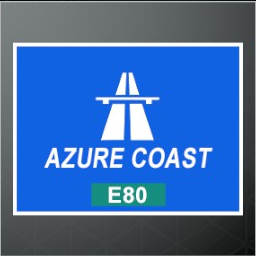
\includegraphics[width=50mm]{LG/2015-05-20_00073.png}
\par Azure Coast\\ France
\end{textblock*}
\begin{textblock*}{80mm}(85mm,15mm)%
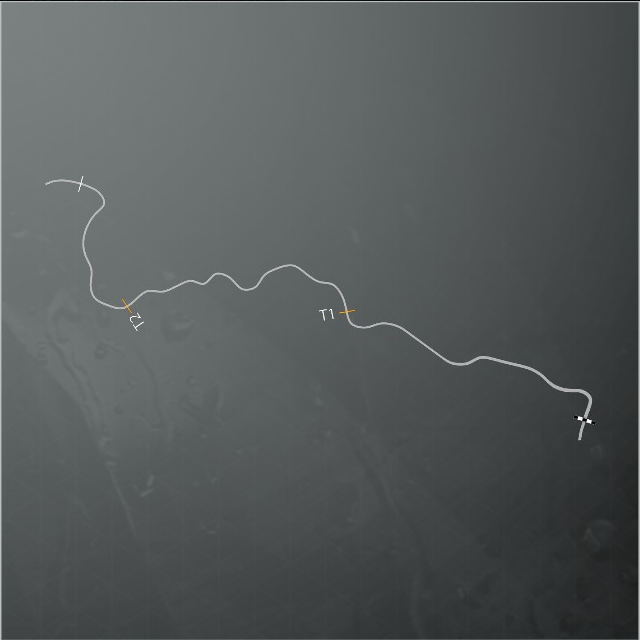
\includegraphics[width=80mm]{TR/2015-05-20_00005.png}
\centerline{Azure Coast Stage 3}
\par\hfill\tiny\tt AZCOS3\\
\end{textblock*}
\begin{textblock*}{30mm}(170mm,15mm)%
\par A $\rightsquigarrow$ B
\Large
\par$\mapsto$ 3.08 mi.
\par$\mapsto$ 4.96 km
\par$\looparrowright$ 22
\end{textblock*}
\begin{textblock*}{80mm}(85mm,105mm)%
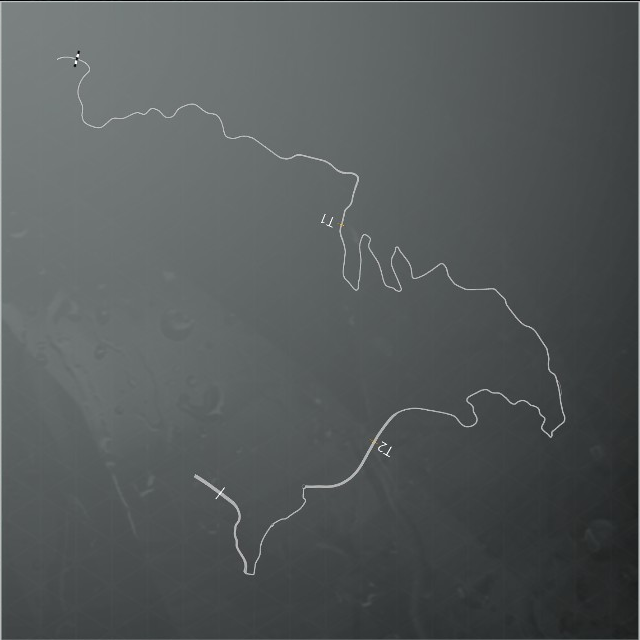
\includegraphics[width=80mm]{TR/2015-05-20_00006.png}
\centerline{Azure Coast Westbound}
\par\hfill\tiny\tt AZCOWE\\
\end{textblock*}
\begin{textblock*}{30mm}(170mm,105mm)%
\par A $\rightsquigarrow$ B
\Large
\par$\mapsto$ 11.97 mi.
\par$\mapsto$ 19.26 km
\par$\looparrowright$ 95
\end{textblock*}
\begin{textblock*}{60mm}(15mm,195mm)%

\includegraphics[width=50mm]{LG/2015-05-20_00087.png}
\par Bathurst\\ Australia
\end{textblock*}
\begin{textblock*}{80mm}(85mm,195mm)%
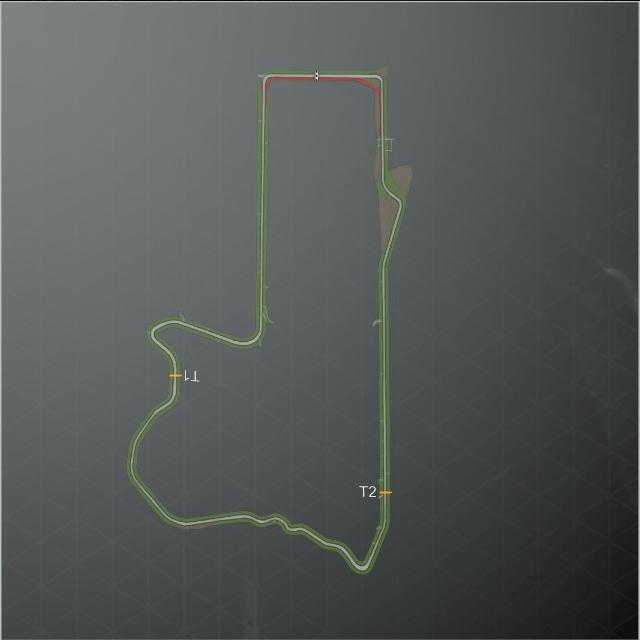
\includegraphics[width=80mm]{TR/2015-05-20_00036.png}
\centerline{Bathurst}
\par\hfill\tiny\tt BA\\
\end{textblock*}
\begin{textblock*}{30mm}(170mm,195mm)%
\par \Huge$\circlearrowleft$
\Large
\par$\mapsto$ 3.86 mi.
\par$\mapsto$ 6.21 km
\par$\looparrowright$ 23
\end{textblock*}
\null\newpage

\begin{textblock*}{60mm}(15mm,15mm)%

\includegraphics[width=50mm]{LG/2015-05-20_00074.png}
\par Brands Hatch\\ United Kingdom
\end{textblock*}
\begin{textblock*}{80mm}(85mm,15mm)%
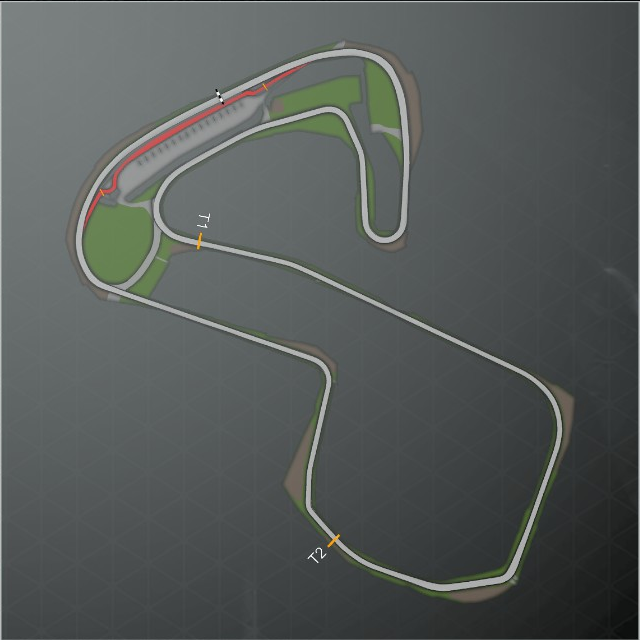
\includegraphics[width=80mm]{TR/2015-05-20_00007.png}
\centerline{Brands Hatch GP}
\par\hfill\tiny\tt BRHAGP\\
\end{textblock*}
\begin{textblock*}{30mm}(170mm,15mm)%
\par \Huge$\circlearrowleft$
\Large
\par$\mapsto$ 2.42 mi.
\par$\mapsto$ 3.89 km
\par$\looparrowright$ 9
\end{textblock*}
\begin{textblock*}{80mm}(85mm,105mm)%
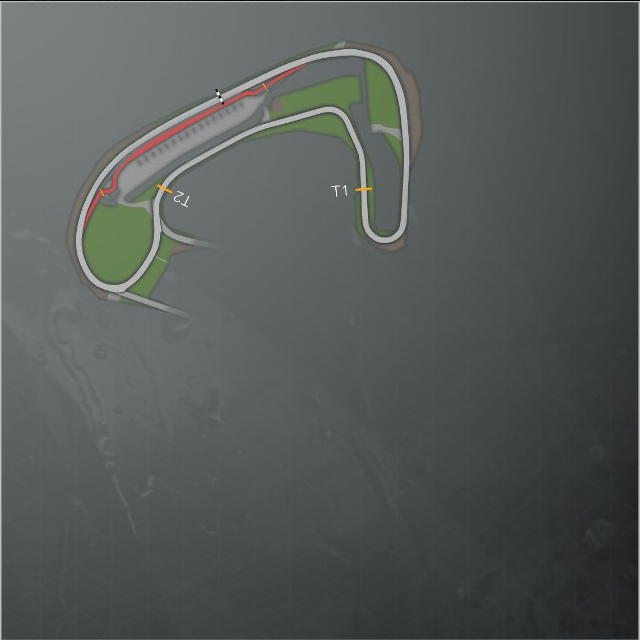
\includegraphics[width=80mm]{TR/2015-05-20_00008.png}
\centerline{Brands Hatch Indy}
\par\hfill\tiny\tt BRHAIN\\
\end{textblock*}
\begin{textblock*}{30mm}(170mm,105mm)%
\par \Huge$\circlearrowleft$
\Large
\par$\mapsto$ 1.19 mi.
\par$\mapsto$ 1.92 km
\par$\looparrowright$ 6
\end{textblock*}
\begin{textblock*}{60mm}(15mm,195mm)%

\includegraphics[width=50mm]{LG/2015-05-20_00075.png}
\par Brno Circuit\\ Czech Republic
\end{textblock*}
\begin{textblock*}{80mm}(85mm,195mm)%
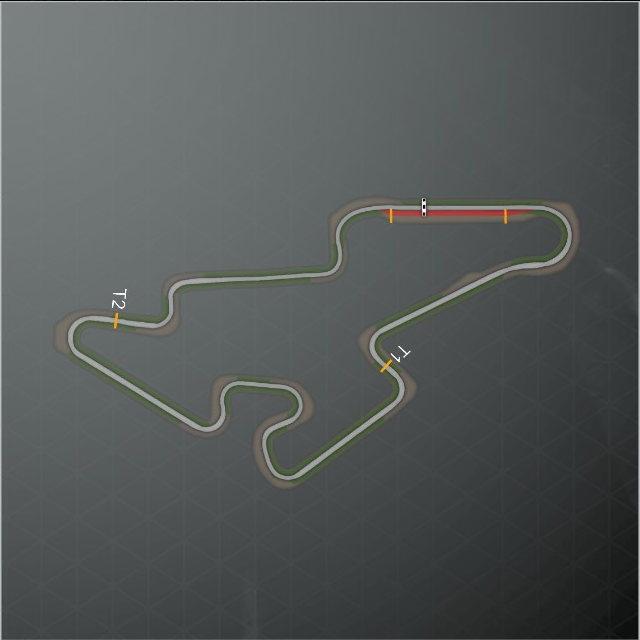
\includegraphics[width=80mm]{TR/2015-05-20_00009.png}
\centerline{Brno}
\par\hfill\tiny\tt BRNO\\
\end{textblock*}
\begin{textblock*}{30mm}(170mm,195mm)%
\par \Huge$\circlearrowleft$
\Large
\par$\mapsto$ 3.35 mi.
\par$\mapsto$ 5.39 km
\par$\looparrowright$ 14
\end{textblock*}
\null\newpage

\begin{textblock*}{60mm}(15mm,15mm)%

\includegraphics[width=50mm]{LG/2015-05-20_00076.png}
\par Cadwell Park\\ United Kingdom
\end{textblock*}
\begin{textblock*}{80mm}(85mm,15mm)%
\includegraphics[width=80mm]{TR/2015-05-20_00011.png}
\centerline{Cadwell Club Circuit}
\par\hfill\tiny\tt CADCLC\\
\end{textblock*}
\begin{textblock*}{30mm}(170mm,15mm)%
\par \Huge$\circlearrowleft$
\Large
\par$\mapsto$ 1.47 mi.
\par$\mapsto$ 2.37 km
\par$\looparrowright$ 7
\end{textblock*}
\begin{textblock*}{80mm}(85mm,105mm)%
\includegraphics[width=80mm]{TR/2015-05-20_00010.png}
\centerline{Cadwell GP}
\par\hfill\tiny\tt CADGP\\
\end{textblock*}
\begin{textblock*}{30mm}(170mm,105mm)%
\par \Huge$\circlearrowleft$
\Large
\par$\mapsto$ 2.16 mi.
\par$\mapsto$ 3.48 km
\par$\looparrowright$ 11
\end{textblock*}
\begin{textblock*}{80mm}(85mm,195mm)%
\includegraphics[width=80mm]{TR/2015-05-20_00012.png}
\centerline{Cadwell Woodland}
\par\hfill\tiny\tt CADWOL\\
\end{textblock*}
\begin{textblock*}{30mm}(170mm,195mm)%
\par \Huge$\circlearrowleft$
\Large
\par$\mapsto$ 0.70 mi.
\par$\mapsto$ 1.13 km
\par$\looparrowright$ 5
\end{textblock*}
\null\newpage

\begin{textblock*}{60mm}(15mm,15mm)%
\includegraphics[width=50mm]{LG/2015-05-20_00077.png}
\par California Highway\\ USA
\end{textblock*}
\begin{textblock*}{80mm}(85mm,15mm)%
\includegraphics[width=80mm]{TR/2015-05-20_00013.png}
\centerline{California Highway Full}
\par\hfill\tiny\tt CAHIFU\\
\end{textblock*}
\begin{textblock*}{30mm}(170mm,15mm)%
\par A $\rightsquigarrow$ B
\Large
\par$\mapsto$ 12.83 mi.
\par$\mapsto$ 20.65 km
\par$\looparrowright$ 107
\end{textblock*}
\begin{textblock*}{80mm}(85mm,105mm)%
\includegraphics[width=80mm]{TR/2015-05-20_00017.png}
\centerline{California Highway Reverse}
\par\hfill\tiny\tt CAHIRE\\
\end{textblock*}
\begin{textblock*}{30mm}(170mm,105mm)%
\par A $\rightsquigarrow$ B
\Large
\par$\mapsto$ 12.83 mi.
\par$\mapsto$ 20.65 km
\par$\looparrowright$ 107
\end{textblock*}
\begin{textblock*}{80mm}(85mm,195mm)%
\includegraphics[width=80mm]{TR/2015-05-20_00014.png}
\centerline{California Highway Stage 1}
\par\hfill\tiny\tt CAHIS1\\
\end{textblock*}
\begin{textblock*}{30mm}(170mm,195mm)%
\par A $\rightsquigarrow$ B
\Large
\par$\mapsto$ 4.11 mi.
\par$\mapsto$ 6.61 km
\par$\looparrowright$ 68
\end{textblock*}
\null\newpage

\begin{textblock*}{60mm}(15mm,15mm)%
\includegraphics[width=50mm]{LG/2015-05-20_00077.png}
\par California Highway\\ USA
\end{textblock*}
\begin{textblock*}{80mm}(85mm,15mm)%
\includegraphics[width=80mm]{TR/2015-05-20_00015.png}
\centerline{California Highway Stage 2}
\par\hfill\tiny\tt CAHIS2\\
\end{textblock*}
\begin{textblock*}{30mm}(170mm,15mm)%
\par A $\rightsquigarrow$ B
\Large
\par$\mapsto$ 5.06 mi.
\par$\mapsto$ 8.14 km
\par$\looparrowright$ 24
\end{textblock*}
\begin{textblock*}{80mm}(85mm,105mm)%
\includegraphics[width=80mm]{TR/2015-05-20_00016.png}
\centerline{California Highway Stage 3}
\par\hfill\tiny\tt CAHIS3\\
\end{textblock*}
\begin{textblock*}{30mm}(170mm,105mm)%
\par A $\rightsquigarrow$ B
\Large
\par$\mapsto$ 3.63 mi.
\par$\mapsto$ 5.84 km
\par$\looparrowright$ 15
\end{textblock*}
\begin{textblock*}{60mm}(15mm,195mm)%
\includegraphics[width=50mm]{LG/2015-05-20_00078.png}
\par Circuit de Barcelona-Catalunya\\ Spain
\end{textblock*}
\begin{textblock*}{80mm}(85mm,195mm)%
\includegraphics[width=80mm]{TR/2015-05-20_00020.png}
\centerline{Circuit de Barcelona-Catalunya Club}
\par\hfill\tiny\tt CBACCL\\
\end{textblock*}
\begin{textblock*}{30mm}(170mm,195mm)%
\par \Huge$\circlearrowleft$
\Large
\par$\mapsto$ 1.05 mi.
\par$\mapsto$ 1.69 km
\par$\looparrowright$ 6
\end{textblock*}
\null\newpage

\begin{textblock*}{60mm}(15mm,15mm)%
\includegraphics[width=50mm]{LG/2015-05-20_00078.png}
\par Circuit de Barcelona-Catalunya\\ Spain
\end{textblock*}
\begin{textblock*}{80mm}(85mm,15mm)%
\includegraphics[width=80mm]{TR/2015-05-20_00018.png}
\centerline{Circuit de Barcelona-Catalunya GP}
\par\hfill\tiny\tt CBACGP\\
\end{textblock*}
\begin{textblock*}{30mm}(170mm,15mm)%
\par \Huge$\circlearrowleft$
\Large
\par$\mapsto$ 2.87 mi.
\par$\mapsto$ 4.62 km
\par$\looparrowright$ 16
\end{textblock*}
\begin{textblock*}{80mm}(85mm,105mm)%
\includegraphics[width=80mm]{TR/2015-05-20_00019.png}
\centerline{Circuit de Barcelona-Catalunya National}
\par\hfill\tiny\tt CBACNA\\
\end{textblock*}
\begin{textblock*}{30mm}(170mm,105mm)%
\par \Huge$\circlearrowleft$
\Large
\par$\mapsto$ 1.90 mi.
\par$\mapsto$ 3.06 km
\par$\looparrowright$ 1
\end{textblock*}
\begin{textblock*}{60mm}(15mm,195mm)%
\includegraphics[width=50mm]{LG/2015-05-20_00079.png}
\par Circuit de Spa-Francorchamps\\ Belgium
\end{textblock*}
\begin{textblock*}{80mm}(85mm,195mm)%
\includegraphics[width=80mm]{TR/2015-05-20_00021.png}
\centerline{Circuit de Spa-Francorchamps}
\par\hfill\tiny\tt CSPAFR\\
\end{textblock*}
\begin{textblock*}{30mm}(170mm,195mm)%
\par \Huge$\circlearrowleft$
\Large
\par$\mapsto$ 4.35 mi.
\par$\mapsto$ 7.00 km
\par$\looparrowright$ 20
\end{textblock*}
\null\newpage

\begin{textblock*}{60mm}(15mm,15mm)%
\includegraphics[width=50mm]{LG/2015-05-20_00084.png}
\par Circuit des 24 Heures du Mans\\ France
\end{textblock*}
\begin{textblock*}{80mm}(85mm,15mm)%
\includegraphics[width=80mm]{TR/2015-05-20_00031.png}
\centerline{Circuit des 24 Heures du Mans}
\par\hfill\tiny\tt CIDUMA\\
\end{textblock*}
\begin{textblock*}{30mm}(170mm,15mm)%
\par \Huge$\circlearrowleft$
\Large
\par$\mapsto$ 8.46 mi.
\par$\mapsto$ 13.62 km
\par$\looparrowright$ 38
\end{textblock*}
\begin{textblock*}{80mm}(85mm,105mm)%
\includegraphics[width=80mm]{TR/2015-05-20_00032.png}
\centerline{Le Circuit Bugatti}
\par\hfill\tiny\tt LECIBU\\
\end{textblock*}
\begin{textblock*}{30mm}(170mm,105mm)%
\par \Huge$\circlearrowleft$
\Large
\par$\mapsto$ 2.65 mi.
\par$\mapsto$ 4.26 km
\par$\looparrowright$ 10
\end{textblock*}
\begin{textblock*}{60mm}(15mm,195mm)%
\includegraphics[width=50mm]{LG/2015-05-20_00080.png}
\par Donington Park\\ United Kingdom
\end{textblock*}
\begin{textblock*}{80mm}(85mm,195mm)%
\includegraphics[width=80mm]{TR/2015-05-20_00022.png}
\centerline{Donington Park GP}
\par\hfill\tiny\tt DOPAGP\\
\end{textblock*}
\begin{textblock*}{30mm}(170mm,195mm)%
\par \Huge$\circlearrowleft$
\Large
\par$\mapsto$ 2.49 mi.
\par$\mapsto$ 4.01 km
\par$\looparrowright$ 12
\end{textblock*}
\null\newpage

\begin{textblock*}{60mm}(15mm,15mm)%
\includegraphics[width=50mm]{LG/2015-05-20_00080.png}
\par Donington Park\\ United Kingdom
\end{textblock*}
\begin{textblock*}{80mm}(85mm,15mm)%
\includegraphics[width=80mm]{TR/2015-05-20_00023.png}
\centerline{Donington Park National}
\par\hfill\tiny\tt DOPANA\\
\end{textblock*}
\begin{textblock*}{30mm}(170mm,15mm)%
\par \Huge$\circlearrowleft$
\Large
\par$\mapsto$ 1.95 mi.
\par$\mapsto$ 3.14 km
\par$\looparrowright$ 10
\end{textblock*}
\begin{textblock*}{60mm}(15mm,105mm)%
\includegraphics[width=50mm]{LG/2015-05-20_00081.png}
\par Dubai Autodrome\\ United Arab Emirates
\end{textblock*}
\begin{textblock*}{80mm}(85mm,105mm)%
\includegraphics[width=80mm]{TR/2015-05-20_00024.png}
\centerline{Dubai Autodrome GP}
\par\hfill\tiny\tt DUAUGP\\
\end{textblock*}
\begin{textblock*}{30mm}(170mm,105mm)%
\par \Huge$\circlearrowleft$
\Large
\par$\mapsto$ 3.31 mi.
\par$\mapsto$ 5.33 km
\par$\looparrowright$ 18
\end{textblock*}
\begin{textblock*}{80mm}(85mm,195mm)%
\includegraphics[width=80mm]{TR/2015-05-20_00026.png}
\centerline{Dubai Autodrome International}
\par\hfill\tiny\tt DUAUIN\\
\end{textblock*}
\begin{textblock*}{30mm}(170mm,195mm)%
\par \Huge$\circlearrowleft$
\Large
\par$\mapsto$ 2.68 mi.
\par$\mapsto$ 4.31 km
\par$\looparrowright$ 12
\end{textblock*}
\null\newpage

\begin{textblock*}{60mm}(15mm,15mm)%
\includegraphics[width=50mm]{LG/2015-05-20_00081.png}
\par Dubai Autodrome\\ United Arab Emirates
\end{textblock*}
\begin{textblock*}{80mm}(85mm,15mm)%
\includegraphics[width=80mm]{TR/2015-05-20_00025.png}
\centerline{Dubai Autodrome National}
\par\hfill\tiny\tt DUAUNA\\
\end{textblock*}
\begin{textblock*}{30mm}(170mm,15mm)%
\par \Huge$\circlearrowleft$
\Large
\par$\mapsto$ 2.23 mi.
\par$\mapsto$ 3.59 km
\par$\looparrowright$ 17
\end{textblock*}
\begin{textblock*}{60mm}(15mm,105mm)%
\includegraphics[width=50mm]{LG/2015-05-20_00082.png}
\par Hockenheim\\ Germany
\end{textblock*}
\begin{textblock*}{80mm}(85mm,105mm)%
\includegraphics[width=80mm]{TR/2015-05-20_00027.png}
\centerline{Hockenheim GP}
\par\hfill\tiny\tt HOGP\\
\end{textblock*}
\begin{textblock*}{30mm}(170mm,105mm)%
\par \Huge$\circlearrowleft$
\Large
\par$\mapsto$ 2.84 mi.
\par$\mapsto$ 4.57 km
\par$\looparrowright$ 17
\end{textblock*}
\begin{textblock*}{80mm}(85mm,195mm)%
\includegraphics[width=80mm]{TR/2015-05-20_00028.png}
\centerline{Hockenheim National}
\par\hfill\tiny\tt HONA\\
\end{textblock*}
\begin{textblock*}{30mm}(170mm,195mm)%
\par \Huge$\circlearrowleft$
\Large
\par$\mapsto$ 2.29 mi.
\par$\mapsto$ 3.69 km
\par$\looparrowright$ 16
\end{textblock*}
\null\newpage

\begin{textblock*}{60mm}(15mm,15mm)%
\includegraphics[width=50mm]{LG/2015-05-20_00082.png}
\par Hockenheim\\ Germany
\end{textblock*}
\begin{textblock*}{80mm}(85mm,15mm)%
\includegraphics[width=80mm]{TR/2015-05-20_00029.png}
\centerline{Hockenheim Short}
\par\hfill\tiny\tt HOSH\\
\end{textblock*}
\begin{textblock*}{30mm}(170mm,15mm)%
\par \Huge$\circlearrowleft$
\Large
\par$\mapsto$ 1.63 mi.
\par$\mapsto$ 2.62 km
\par$\looparrowright$ 14
\end{textblock*}
\begin{textblock*}{60mm}(15mm,105mm)%
\includegraphics[width=50mm]{LG/2015-05-20_00083.png}
\par Imola\\ Italy
\end{textblock*}
\begin{textblock*}{80mm}(85mm,105mm)%
\includegraphics[width=80mm]{TR/2015-05-20_00030.png}
\centerline{Imola}
\par\hfill\tiny\tt IMOL\\
\end{textblock*}
\begin{textblock*}{30mm}(170mm,105mm)%
\par \Huge$\circlearrowleft$
\Large
\par$\mapsto$ 3.05 mi.
\par$\mapsto$ 4.91 km
\par$\looparrowright$ 17
\end{textblock*}
\begin{textblock*}{60mm}(15mm,195mm)%
\includegraphics[width=50mm]{LG/2015-05-20_00085.png}
\par Mazda Raceway Laguna Seca\\ USA
\end{textblock*}
\begin{textblock*}{80mm}(85mm,195mm)%
\includegraphics[width=80mm]{TR/2015-05-21_00001.png}
\centerline{Mazda Raceway Laguna Seca}
\par\hfill\tiny\tt MRLASE\\
\end{textblock*}
\begin{textblock*}{30mm}(170mm,195mm)%
\par \Huge$\circlearrowleft$
\Large
\par$\mapsto$ 2.23 mi.
\par$\mapsto$ 3.59 km
\par$\looparrowright$ 11
\end{textblock*}
\null\newpage

\begin{textblock*}{60mm}(15mm,15mm)%
\includegraphics[width=50mm]{LG/2015-05-20_00088.png}
\par Nordschleife\\ Germany
\end{textblock*}
\begin{textblock*}{80mm}(85mm,15mm)%
\includegraphics[width=80mm]{TR/2015-05-20_00037.png}
\centerline{Nordschleife}
\par\hfill\tiny\tt NO\\
\end{textblock*}
\begin{textblock*}{30mm}(170mm,15mm)%
\par \Huge$\circlearrowleft$
\Large
\par$\mapsto$ 12.94 mi.
\par$\mapsto$ 20.82 km
\par$\looparrowright$ 73
\end{textblock*}
\begin{textblock*}{80mm}(85mm,105mm)%
\includegraphics[width=80mm]{TR/2015-05-20_00038.png}
\centerline{Nordschleife Stage 1}
\par\hfill\tiny\tt NOS1\\
\end{textblock*}
\begin{textblock*}{30mm}(170mm,105mm)%
\par A $\rightsquigarrow$ B
\Large
\par$\mapsto$ 4.29 mi.
\par$\mapsto$ 6.90 km
\par$\looparrowright$ 36
\end{textblock*}
\begin{textblock*}{80mm}(85mm,195mm)%
\includegraphics[width=80mm]{TR/2015-05-20_00039.png}
\centerline{Nordschleife Stage 2}
\par\hfill\tiny\tt NOS2\\
\end{textblock*}
\begin{textblock*}{30mm}(170mm,195mm)%
\par A $\rightsquigarrow$ B
\Large
\par$\mapsto$ 3.70 mi.
\par$\mapsto$ 5.95 km
\par$\looparrowright$ 33
\end{textblock*}
\null\newpage

\begin{textblock*}{60mm}(15mm,15mm)%
\includegraphics[width=50mm]{LG/2015-05-20_00088.png}
\par Nordschleife\\ Germany
\end{textblock*}
\begin{textblock*}{80mm}(85mm,15mm)%
\includegraphics[width=80mm]{TR/2015-05-20_00040.png}
\centerline{Nordschleife Stage 3}
\par\hfill\tiny\tt NOS3\\
\end{textblock*}
\begin{textblock*}{30mm}(170mm,15mm)%
\par A $\rightsquigarrow$ B
\Large
\par$\mapsto$ 4.89 mi.
\par$\mapsto$ 7.87 km
\par$\looparrowright$ 44
\end{textblock*}
\begin{textblock*}{60mm}(15mm,105mm)%
\includegraphics[width=50mm]{LG/2015-05-20_00089.png}
\par Nürburgring\\ Germany
\end{textblock*}
\begin{textblock*}{80mm}(85mm,105mm)%
\includegraphics[width=80mm]{TR/2015-05-20_00041.png}
\centerline{Nürburgring GP}
\par\hfill\tiny\tt NBRGP\\
\end{textblock*}
\begin{textblock*}{30mm}(170mm,105mm)%
\par \Huge$\circlearrowleft$
\Large
\par$\mapsto$ 3.19 mi.
\par$\mapsto$ 5.13 km
\par$\looparrowright$ 16
\end{textblock*}
\begin{textblock*}{80mm}(85mm,195mm)%
\includegraphics[width=80mm]{TR/2015-05-20_00042.png}
\centerline{Nürburgring Müllenbach}
\par\hfill\tiny\tt NBRMB\\
\end{textblock*}
\begin{textblock*}{30mm}(170mm,195mm)%
\par \Huge$\circlearrowleft$
\Large
\par$\mapsto$ 0.92 mi.
\par$\mapsto$ 1.48 km
\par$\looparrowright$ 8
\end{textblock*}
\null\newpage

\begin{textblock*}{60mm}(15mm,15mm)%
\includegraphics[width=50mm]{LG/2015-05-20_00089.png}
\par Nürburgring\\ Germany
\end{textblock*}
\begin{textblock*}{80mm}(85mm,15mm)%
\includegraphics[width=80mm]{TR/2015-05-20_00043.png}
\centerline{Nürburgring Sprint}
\par\hfill\tiny\tt NBRSP\\
\end{textblock*}
\begin{textblock*}{30mm}(170mm,15mm)%
\par \Huge$\circlearrowleft$
\Large
\par$\mapsto$ 2.25 mi.
\par$\mapsto$ 3.62 km
\par$\looparrowright$ 11
\end{textblock*}
\begin{textblock*}{80mm}(85mm,105mm)%
\includegraphics[width=80mm]{TR/2015-05-20_00044.png}
\centerline{Nürburgring Sprint Short}
\par\hfill\tiny\tt NBRSPS\\
\end{textblock*}
\begin{textblock*}{30mm}(170mm,105mm)%
\par \Huge$\circlearrowleft$
\Large
\par$\mapsto$ 1.90 mi.
\par$\mapsto$ 3.06 km
\par$\looparrowright$ 9
\end{textblock*}
\begin{textblock*}{60mm}(15mm,195mm)%
\includegraphics[width=50mm]{LG/2015-05-20_00090.png}
\par Oschersleben\\ Germany
\end{textblock*}
\begin{textblock*}{80mm}(85mm,195mm)%
\includegraphics[width=80mm]{TR/2015-05-20_00047.png}
\centerline{Oschersleben C Circuit}
\par\hfill\tiny\tt OSCI\\
\end{textblock*}
\begin{textblock*}{30mm}(170mm,195mm)%
\par \Huge$\circlearrowleft$
\Large
\par$\mapsto$ 0.68 mi.
\par$\mapsto$ 1.09 km
\par$\looparrowright$ 8
\end{textblock*}
\null\newpage

\begin{textblock*}{60mm}(15mm,15mm)%
\includegraphics[width=50mm]{LG/2015-05-20_00090.png}
\par Oschersleben\\ Germany
\end{textblock*}
\begin{textblock*}{80mm}(85mm,15mm)%
\includegraphics[width=80mm]{TR/2015-05-20_00045.png}
\centerline{Oschersleben GP}
\par\hfill\tiny\tt OSGP\\
\end{textblock*}
\begin{textblock*}{30mm}(170mm,15mm)%
\par \Huge$\circlearrowleft$
\Large
\par$\mapsto$ 2.27 mi.
\par$\mapsto$ 3.65 km
\par$\looparrowright$ 15
\end{textblock*}
\begin{textblock*}{80mm}(85mm,105mm)%
\includegraphics[width=80mm]{TR/2015-05-20_00046.png}
\centerline{Oschersleben National}
\par\hfill\tiny\tt OSNA\\
\end{textblock*}
\begin{textblock*}{30mm}(170mm,105mm)%
\par \Huge$\circlearrowleft$
\Large
\par$\mapsto$ 1.51 mi.
\par$\mapsto$ 2.43 km
\par$\looparrowright$ 8
\end{textblock*}
\begin{textblock*}{60mm}(15mm,195mm)%
\includegraphics[width=50mm]{LG/2015-05-20_00091.png}
\par Oulton Park\\ United Kingdom
\end{textblock*}
\begin{textblock*}{80mm}(85mm,195mm)%
\includegraphics[width=80mm]{TR/2015-05-20_00050.png}
\centerline{Oulton Park Fosters}
\par\hfill\tiny\tt OUPAFO\\
\end{textblock*}
\begin{textblock*}{30mm}(170mm,195mm)%
\par \Huge$\circlearrowleft$
\Large
\par$\mapsto$ 1.65 mi.
\par$\mapsto$ 2.66 km
\par$\looparrowright$ 5
\end{textblock*}
\null\newpage

\begin{textblock*}{60mm}(15mm,15mm)%
\includegraphics[width=50mm]{LG/2015-05-20_00091.png}
\par Oulton Park\\ United Kingdom
\end{textblock*}
\begin{textblock*}{80mm}(85mm,15mm)%
\includegraphics[width=80mm]{TR/2015-05-20_00048.png}
\centerline{Oulton Park International}
\par\hfill\tiny\tt OUPAIN\\
\end{textblock*}
\begin{textblock*}{30mm}(170mm,15mm)%
\par \Huge$\circlearrowleft$
\Large
\par$\mapsto$ 2.67 mi.
\par$\mapsto$ 4.30 km
\par$\looparrowright$ 17
\end{textblock*}
\begin{textblock*}{80mm}(85mm,105mm)%
\includegraphics[width=80mm]{TR/2015-05-20_00049.png}
\centerline{Oulton Park Island}
\par\hfill\tiny\tt OUPAIS\\
\end{textblock*}
\begin{textblock*}{30mm}(170mm,105mm)%
\par \Huge$\circlearrowleft$
\Large
\par$\mapsto$ 2.24 mi.
\par$\mapsto$ 3.60 km
\par$\looparrowright$ 7
\end{textblock*}
\begin{textblock*}{60mm}(15mm,195mm)%
\includegraphics[width=50mm]{LG/2015-05-20_00092.png}
\par Road America\\ USA
\end{textblock*}
\begin{textblock*}{80mm}(85mm,195mm)%
\includegraphics[width=80mm]{TR/2015-05-20_00051.png}
\centerline{Road America}
\par\hfill\tiny\tt ROAM\\
\end{textblock*}
\begin{textblock*}{30mm}(170mm,195mm)%
\par \Huge$\circlearrowleft$
\Large
\par$\mapsto$ 4.04 mi.
\par$\mapsto$ 6.50 km
\par$\looparrowright$ 14
\end{textblock*}
\null\newpage

\begin{textblock*}{60mm}(15mm,15mm)%
\includegraphics[width=50mm]{LG/2015-05-20_00093.png}
\par Sakitto\\ Japan
\end{textblock*}
\begin{textblock*}{80mm}(85mm,15mm)%
\includegraphics[width=80mm]{TR/2015-05-20_00052.png}
\centerline{Sakitto GP}
\par\hfill\tiny\tt SAGP\\
\end{textblock*}
\begin{textblock*}{30mm}(170mm,15mm)%
\par \Huge$\circlearrowleft$
\Large
\par$\mapsto$ 3.34 mi.
\par$\mapsto$ 5.38 km
\par$\looparrowright$ 15
\end{textblock*}
\begin{textblock*}{80mm}(85mm,105mm)%
\includegraphics[width=80mm]{TR/2015-05-20_00055.png}
\centerline{Sakitto International}
\par\hfill\tiny\tt SAIN\\
\end{textblock*}
\begin{textblock*}{30mm}(170mm,105mm)%
\par \Huge$\circlearrowleft$
\Large
\par$\mapsto$ 1.76 mi.
\par$\mapsto$ 2.83 km
\par$\looparrowright$ 12
\end{textblock*}
\begin{textblock*}{80mm}(85mm,195mm)%
\includegraphics[width=80mm]{TR/2015-05-20_00054.png}
\centerline{Sakitto National}
\par\hfill\tiny\tt SANA\\
\end{textblock*}
\begin{textblock*}{30mm}(170mm,195mm)%
\par \Huge$\circlearrowleft$
\Large
\par$\mapsto$ 1.92 mi.
\par$\mapsto$ 3.09 km
\par$\looparrowright$ 12
\end{textblock*}
\null\newpage

\begin{textblock*}{60mm}(15mm,15mm)%
\includegraphics[width=50mm]{LG/2015-05-20_00093.png}
\par Sakitto\\ Japan
\end{textblock*}
\begin{textblock*}{80mm}(85mm,15mm)%
\includegraphics[width=80mm]{TR/2015-05-20_00053.png}
\centerline{Sakitto Sprint}
\par\hfill\tiny\tt SASP\\
\end{textblock*}
\begin{textblock*}{30mm}(170mm,15mm)%
\par \Huge$\circlearrowleft$
\Large
\par$\mapsto$ 2.19 mi.
\par$\mapsto$ 3.52 km
\par$\looparrowright$ 14
\end{textblock*}
\begin{textblock*}{60mm}(15mm,105mm)%
\includegraphics[width=50mm]{LG/2015-05-20_00094.png}
\par Silverstone\\ United Kingdom
\end{textblock*}
\begin{textblock*}{80mm}(85mm,105mm)%
\includegraphics[width=80mm]{TR/2015-05-20_00056.png}
\centerline{Silverstone GP}
\par\hfill\tiny\tt SIGP\\
\end{textblock*}
\begin{textblock*}{30mm}(170mm,105mm)%
\par \Huge$\circlearrowleft$
\Large
\par$\mapsto$ 3.66 mi.
\par$\mapsto$ 5.89 km
\par$\looparrowright$ 18
\end{textblock*}
\begin{textblock*}{80mm}(85mm,195mm)%
\includegraphics[width=80mm]{TR/2015-05-20_00057.png}
\centerline{Silverstone International}
\par\hfill\tiny\tt SIIN\\
\end{textblock*}
\begin{textblock*}{30mm}(170mm,195mm)%
\par \Huge$\circlearrowleft$
\Large
\par$\mapsto$ 2.24 mi.
\par$\mapsto$ 3.60 km
\par$\looparrowright$ 10
\end{textblock*}
\null\newpage

\begin{textblock*}{60mm}(15mm,15mm)%
\includegraphics[width=50mm]{LG/2015-05-20_00094.png}
\par Silverstone\\ United Kingdom
\end{textblock*}
\begin{textblock*}{80mm}(85mm,15mm)%
\includegraphics[width=80mm]{TR/2015-05-20_00058.png}
\centerline{Silverstone National}
\par\hfill\tiny\tt SINA\\
\end{textblock*}
\begin{textblock*}{30mm}(170mm,15mm)%
\par \Huge$\circlearrowleft$
\Large
\par$\mapsto$ 1.63 mi.
\par$\mapsto$ 2.62 km
\par$\looparrowright$ 6
\end{textblock*}
\begin{textblock*}{80mm}(85mm,105mm)%
\includegraphics[width=80mm]{TR/2015-05-20_00059.png}
\centerline{Silverstone Stowe}
\par\hfill\tiny\tt SIST\\
\end{textblock*}
\begin{textblock*}{30mm}(170mm,105mm)%
\par \Huge$\circlearrowleft$
\Large
\par$\mapsto$ 0.79 mi.
\par$\mapsto$ 1.27 km
\par$\looparrowright$ 16
\end{textblock*}
\begin{textblock*}{60mm}(15mm,195mm)%
\includegraphics[width=50mm]{LG/2015-05-20_00095.png}
\par Snetterton\\ United Kingdom
\end{textblock*}
\begin{textblock*}{80mm}(85mm,195mm)%
\includegraphics[width=80mm]{TR/2015-05-20_00062.png}
\centerline{Snetterton 100}
\par\hfill\tiny\tt SN100\\
\end{textblock*}
\begin{textblock*}{30mm}(170mm,195mm)%
\par \Huge$\circlearrowleft$
\Large
\par$\mapsto$ 0.98 mi.
\par$\mapsto$ 1.58 km
\par$\looparrowright$ 6
\end{textblock*}
\null\newpage

\begin{textblock*}{60mm}(15mm,15mm)%
\includegraphics[width=50mm]{LG/2015-05-20_00095.png}
\par Snetterton\\ United Kingdom
\end{textblock*}
\begin{textblock*}{80mm}(85mm,15mm)%
\includegraphics[width=80mm]{TR/2015-05-20_00061.png}
\centerline{Snetterton 200}
\par\hfill\tiny\tt SN200\\
\end{textblock*}
\begin{textblock*}{30mm}(170mm,15mm)%
\par \Huge$\circlearrowleft$
\Large
\par$\mapsto$ 2.00 mi.
\par$\mapsto$ 3.22 km
\par$\looparrowright$ 8
\end{textblock*}
\begin{textblock*}{80mm}(85mm,105mm)%
\includegraphics[width=80mm]{TR/2015-05-20_00060.png}
\centerline{Snetterton 300}
\par\hfill\tiny\tt SN300\\
\end{textblock*}
\begin{textblock*}{30mm}(170mm,105mm)%
\par \Huge$\circlearrowleft$
\Large
\par$\mapsto$ 2.96 mi.
\par$\mapsto$ 4.76 km
\par$\looparrowright$ 13
\end{textblock*}
\begin{textblock*}{60mm}(15mm,195mm)%
\includegraphics[width=50mm]{LG/2015-05-20_00096.png}
\par Sonoma Raceway\\ USA
\end{textblock*}
\begin{textblock*}{80mm}(85mm,195mm)%
\includegraphics[width=80mm]{TR/2015-05-20_00065.png}
\centerline{Sonoma Raceway GP}
\par\hfill\tiny\tt SORAGP\\
\end{textblock*}
\begin{textblock*}{30mm}(170mm,195mm)%
\par \Huge$\circlearrowleft$
\Large
\par$\mapsto$ 2.51 mi.
\par$\mapsto$ 4.04 km
\par$\looparrowright$ 19
\end{textblock*}
\null\newpage

\begin{textblock*}{60mm}(15mm,15mm)%
\includegraphics[width=50mm]{LG/2015-05-20_00096.png}
\par Sonoma Raceway\\ USA
\end{textblock*}
\begin{textblock*}{80mm}(85mm,15mm)%
\includegraphics[width=80mm]{TR/2015-05-20_00064.png}
\centerline{Sonoma Raceway National}
\par\hfill\tiny\tt SORANA\\
\end{textblock*}
\begin{textblock*}{30mm}(170mm,15mm)%
\par \Huge$\circlearrowleft$
\Large
\par$\mapsto$ 2.29 mi.
\par$\mapsto$ 3.69 km
\par$\looparrowright$ 17
\end{textblock*}
\begin{textblock*}{80mm}(85mm,105mm)%
\includegraphics[width=80mm]{TR/2015-05-20_00063.png}
\centerline{Sonoma Raceway Short}
\par\hfill\tiny\tt SORASH\\
\end{textblock*}
\begin{textblock*}{30mm}(170mm,105mm)%
\par \Huge$\circlearrowleft$
\Large
\par$\mapsto$ 1.94 mi.
\par$\mapsto$ 3.12 km
\par$\looparrowright$ 15
\end{textblock*}
\begin{textblock*}{60mm}(15mm,195mm)%
\includegraphics[width=50mm]{LG/2015-05-20_00097.png}
\par Watkins Glen\\ USA
\end{textblock*}
\begin{textblock*}{80mm}(85mm,195mm)%
\includegraphics[width=80mm]{TR/2015-05-20_00066.png}
\centerline{Watkins Glen GP}
\par\hfill\tiny\tt WAGLGP\\
\end{textblock*}
\begin{textblock*}{30mm}(170mm,195mm)%
\par \Huge$\circlearrowleft$
\Large
\par$\mapsto$ 3.37 mi.
\par$\mapsto$ 5.42 km
\par$\looparrowright$ 11
\end{textblock*}
\null\newpage

\begin{textblock*}{60mm}(15mm,15mm)%
\includegraphics[width=50mm]{LG/2015-05-20_00097.png}
\par Watkins Glen\\ USA
\end{textblock*}
\begin{textblock*}{80mm}(85mm,15mm)%
\includegraphics[width=80mm]{TR/2015-05-20_00067.png}
\centerline{Watkins Glen Short}
\par\hfill\tiny\tt WAGLSH\\
\end{textblock*}
\begin{textblock*}{30mm}(170mm,15mm)%
\par \Huge$\circlearrowleft$
\Large
\par$\mapsto$ 2.52 mi.
\par$\mapsto$ 4.06 km
\par$\looparrowright$ 8
\end{textblock*}
\begin{textblock*}{60mm}(15mm,105mm)%
\includegraphics[width=50mm]{LG/2015-05-20_00098.png}
\par Willow Springs\\ USA
\end{textblock*}
\begin{textblock*}{80mm}(85mm,105mm)%
\includegraphics[width=80mm]{TR/2015-05-20_00069.png}
\centerline{Willow Springs Horse Thief Mile}
\par\hfill\tiny\tt WSPHTM\\
\end{textblock*}
\begin{textblock*}{30mm}(170mm,105mm)%
\par \Huge$\circlearrowleft$
\Large
\par$\mapsto$ 0.99 mi.
\par$\mapsto$ 1.59 km
\par$\looparrowright$ 11
\end{textblock*}
\begin{textblock*}{80mm}(85mm,195mm)%
\includegraphics[width=80mm]{TR/2015-05-20_00068.png}
\centerline{Willow Springs International Raceway}
\par\hfill\tiny\tt WSPIR\\
\end{textblock*}
\begin{textblock*}{30mm}(170mm,195mm)%
\par \Huge$\circlearrowleft$
\Large
\par$\mapsto$ 2.49 mi.
\par$\mapsto$ 4.01 km
\par$\looparrowright$ 9
\end{textblock*}
\null\newpage

\begin{textblock*}{60mm}(15mm,15mm)%
\includegraphics[width=50mm]{LG/2015-05-20_00100.png}
\par Zolder\\ Belgium
\end{textblock*}
\begin{textblock*}{80mm}(85mm,15mm)%
\includegraphics[width=80mm]{TR/2015-05-20_00071.png}
\centerline{Zolder}
\par\hfill\tiny\tt ZO\\
\end{textblock*}
\begin{textblock*}{30mm}(170mm,15mm)%
\par \Huge$\circlearrowleft$
\Large
\par$\mapsto$ 2.49 mi.
\par$\mapsto$ 4.01 km
\par$\looparrowright$ 10
\end{textblock*}
\begin{textblock*}{60mm}(15mm,105mm)%
\includegraphics[width=50mm]{LG/2015-05-20_00099.png}
\par Zuhai International\\ China
\end{textblock*}
\begin{textblock*}{80mm}(85mm,105mm)%
\includegraphics[width=80mm]{TR/2015-05-20_00070.png}
\centerline{Zuhai International Circuit}
\par\hfill\tiny\tt ZUIC\\
\end{textblock*}
\begin{textblock*}{30mm}(170mm,105mm)%
\par \Huge$\circlearrowleft$
\Large
\par$\mapsto$ 2.68 mi.
\par$\mapsto$ 4.31 km
\par$\looparrowright$ 14
\end{textblock*}



\end{document}
